% Appendix Template

\chapter{Results of experiment 2.8} % Main appendix title

\label{Appendix2-8} % Change X to a consecutive letter; for referencing this appendix elsewhere, use \ref{AppendixX}

\begin{figure}[ht]
  \centering
  \begin{subfigure}[b]{0.5\linewidth}
    \centering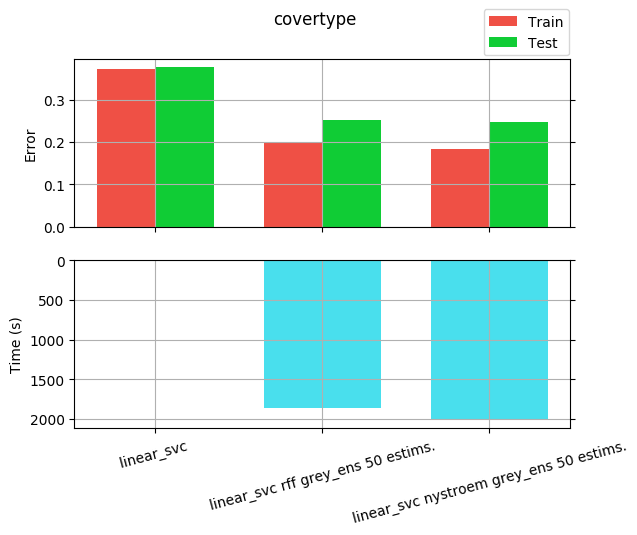
\includegraphics[width=\imgscale\linewidth]{Figures/2_8/covertype}
    \caption{prueba covertype}
    \label{fig:2_8_covertype}
  \end{subfigure}%
  \begin{subfigure}[b]{0.5\linewidth}
    \centering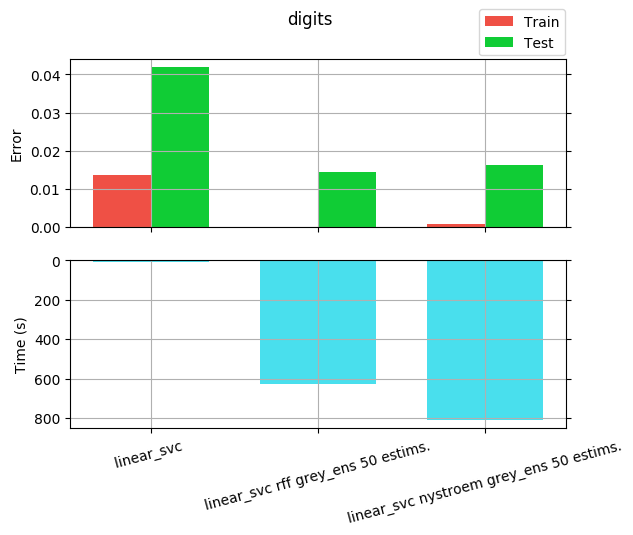
\includegraphics[width=\imgscale\linewidth]{Figures/2_8/digits}
    \caption{prueba digits}
    \label{fig:2_8_digits}
  \end{subfigure}
\end{figure}


\begin{figure}[ht]
  \centering
  \begin{subfigure}[b]{0.5\linewidth}
    \centering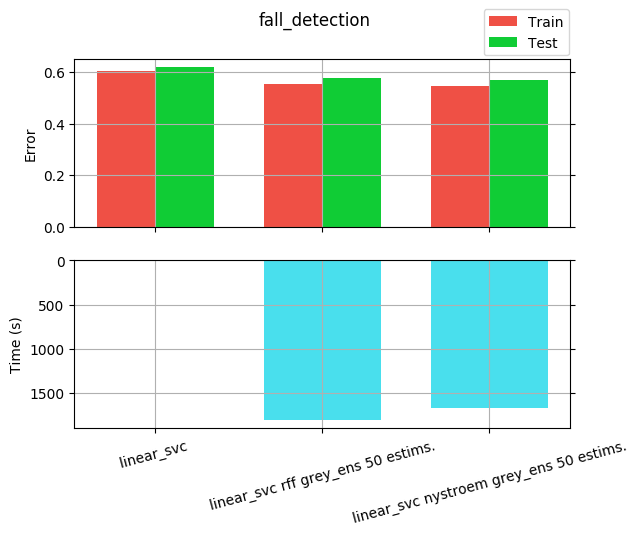
\includegraphics[width=\imgscale\linewidth]{Figures/2_8/fall_detection}
    \caption{prueba fall-detection}
    \label{fig:2_8_fall_detection}
  \end{subfigure}%
  \begin{subfigure}[b]{0.5\linewidth}
    \centering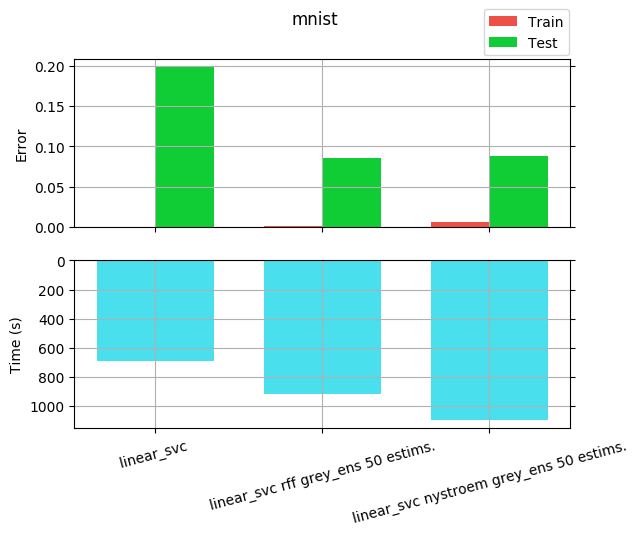
\includegraphics[width=\imgscale\linewidth]{Figures/2_8/mnist}
    \caption{prueba mnist}
    \label{fig:2_8_mnist}
  \end{subfigure}
\end{figure}


\begin{figure}[ht]
  \centering
  \begin{subfigure}[b]{0.5\linewidth}
    \centering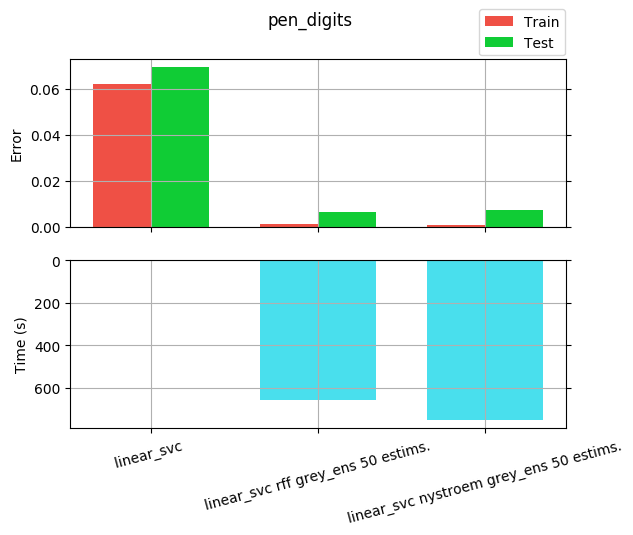
\includegraphics[width=\imgscale\linewidth]{Figures/2_8/pen_digits}
    \caption{prueba pen-digits}
    \label{fig:2_8_pen_digits}
  \end{subfigure}%
  \begin{subfigure}[b]{0.5\linewidth}
    \centering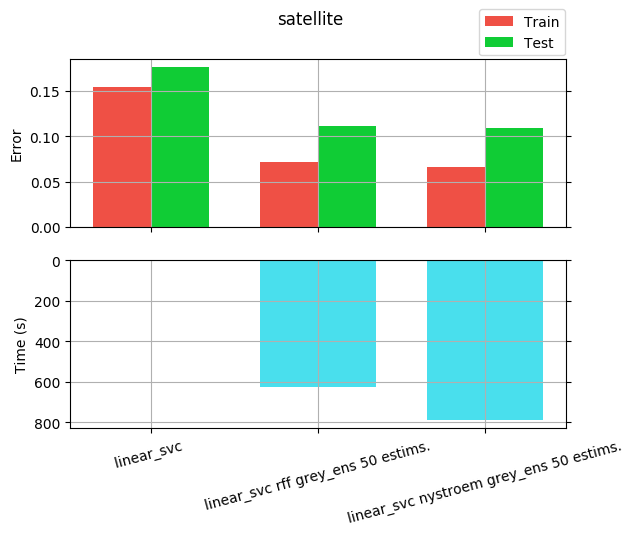
\includegraphics[width=\imgscale\linewidth]{Figures/2_8/satellite}
    \caption{prueba satellite}
    \label{fig:2_8_satellite}
  \end{subfigure}
\end{figure}

\begin{figure}[ht]
  \centering
  \begin{subfigure}[b]{0.5\linewidth}
    \centering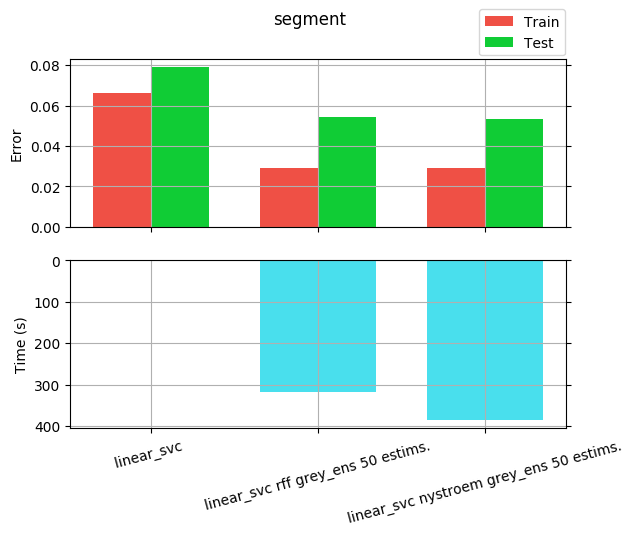
\includegraphics[width=\imgscale\linewidth]{Figures/2_8/segment}
    \caption{prueba segment}
    \label{fig:2_8_segment}
  \end{subfigure}%
  \begin{subfigure}[b]{0.5\linewidth}
    \centering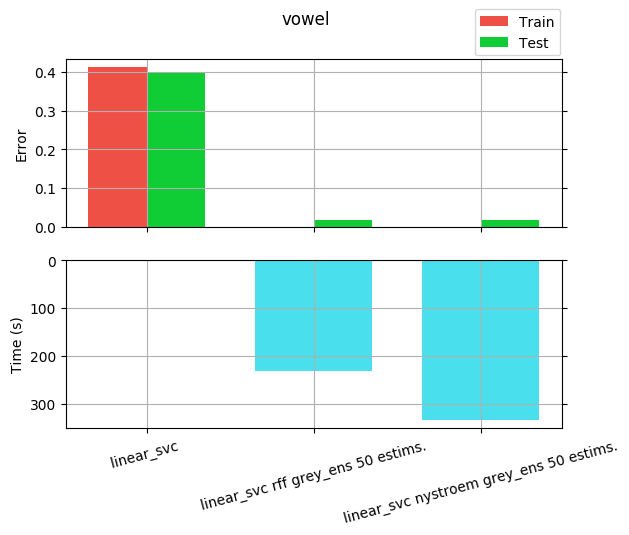
\includegraphics[width=\imgscale\linewidth]{Figures/2_8/vowel}
    \caption{prueba vowel}
    \label{fig:2_8_vowel}
  \end{subfigure}
\end{figure}
